
\subsection{Delay public release} \label{sec:3delay}

Rubin considers the best approach to managing public release of data is to keep the embargoed data on a secure device separate from other systems and migrate images to the regular repository as they become \emph{public}.
This can be an object store with encryption like MinIO \footnote{\url{ https://min.io/product/enterprise-object-storage-encryption}}.
We will need to have one at \gls{SLAC} and one at Chile for redundancy to ensure no data loss.

With the commissioning constraint that means this needs to be approximately a one month store  for full images and engineering data.
Looking at \citeds{DMTN-135}
table 40 this comes out to about 500TB of usable disk.
\tabref{tab:delay} gives the cost calculation or this.

The nominal embargo for regular operations we understand as between a few days (most images) and ten days (some images as specified by \gls{Alert} Vetting).

\tiny \begin{longtable} {|p{0.3\textwidth}|r|l|} \caption{This table provides costs for the embargoed data store.  \label{tab:delay}}\\ 
\hline 
\textbf{Description}&\textbf{value}& \\ \hline
{Number of days data to store}&{30}& \\ \hline
{Raw data size per day (TB compressed)}&{16}&{Years data from Table 40 of \citeds{DMTN-135}\/ 298.3 observing nights (Key Numbers Confluence) } \\ \hline
{Useable size needed (TB)}&{484}& \\ \hline
{Allowing for RAID (TB)}&{1000}& \\ \hline
{Cost for 1 store}&{\$400,000}&{Using SLAC Fast Disk Price from Table 28 of \citeds{DMTN-135}} \\ \hline
\textbf{Total for 2 stores}&\textbf{\$800,000}& \\ \hline
{Ops Cost at least 1 Refresh}&{\$800,000}& \\ \hline
\end{longtable} \normalsize



{\bf Note:} To enact these enhanced security measures on \gls{Commissioning} data, this plan focuses on early data processing at the SLAC USDF and not the resources originally planned at NCSA. The SLAC USDF must be ready with sufficient services and capacity for ComCam, on sky work.

\figref{fig:arch} depicts the encrypted storage and network. Embargoed (delayed) data would be held in the encrypted stores for the time specified.
We assume temporary processing for alerts does not have to be encrypted, \gls{NIST} allows ephemeral unencrypted data for processing.

\begin{figure}
\begin{centering}
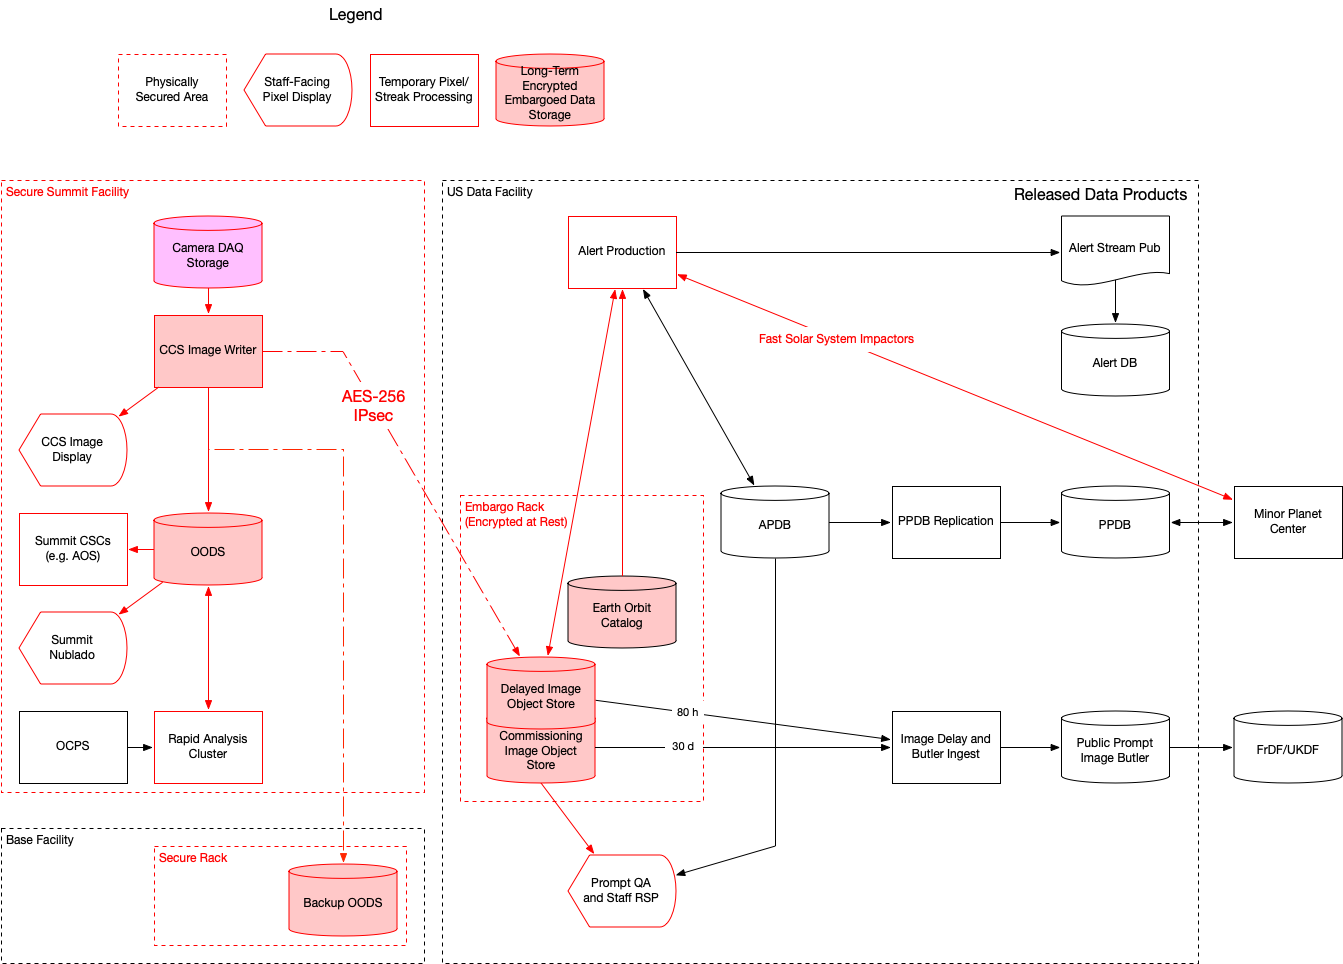
\includegraphics[width=\textwidth]{Embargo_arch}
	\caption{ Architecture diagram showing many details including the long term encrypted storage and encrypted network from Chile to SLAC. \label{fig:arch}}
\end{centering}
\end{figure}
